\documentclass[12pt]{article}
\usepackage{amsmath}
\usepackage{amsthm}
\usepackage{amssymb}
\usepackage{geometry}
\usepackage{enumitem}
\usepackage{booktabs}
\usepackage{graphicx}
\usepackage{hyperref}

\usepackage{appendix}

\geometry{margin=2.5cm}

\newtheorem{proposition}{Proposition}
\newtheorem{theorem}{Theorem}
\newtheorem{remark}{Remark}
\newtheorem{conjecture}{Conjecture}
\newtheorem{corollary}{Corollary}[section]
\newtheorem{assumption}{Assumption}

\title{A Structural Model of Rational Addiction}
\author{Yushang Cheng\\
  \small\texttt{1302573502@qq.com}\\
  \small\href{https://orcid.org/0009-0001-3218-6423}{\textsc{orcid}: 0009-0001-3218-6423}}
\date{May 19, 2026}

\begin{document}
\maketitle

\begin{abstract}
Building on the Becker-Murphy (1988) framework, this paper introduces two complementary variables that further develop the original theory.
One of these variables is an original exit mechanism, representing the consistency value an addict obtains from transitioning toward their ideal state.
Quadratic adjustment friction captures the physiological and psychological costs of changing consumption habits, while the exit mechanism (a utility function represented by a family of integral-form functions)
transforms withdrawal behavior from a pure welfare loss into an active choice.
I employ dynamic programming to derive optimality conditions, characterize multiple steady states,
and conduct comparative static analysis. A key finding after introducing these two new variables is that the interaction between adjustment friction and the exit mechanism
generates complex roots in the Euler system, making relapse paths compatible with the necessary conditions for rational optimality (the Euler equation and transversality condition).
The linearized Euler equation connects theory with survey-based estimates and remains compatible with Chaloupka (1991) and Becker et al. (1994).
\end{abstract}

\textbf{Keywords}: Rational addiction, habit formation, adjustment friction, exit mechanism, relapse, dynamic programming.

\textbf{JEL Codes}: D11, D90, I12.

\section{Introduction}

The economic analysis of addiction has been decisively shaped by the rational addiction model of Becker and Murphy (1988). Unlike
views that treat addicts as impulsive or irrational, Becker and Murphy argue that even severe addictive behavior can
be understood as the result of consistent and forward-looking utility maximization. The key mechanism is reinforcement: past consumption raises the
marginal utility of current consumption, making the two adjacent complements. This generates multiple steady states, cold-turkey withdrawal,
and stronger demand sensitivity to permanent price changes than to temporary price changes.

Existing literature extends the Becker-Murphy framework from multiple angles. Orphanides and Zervos \cite{Orphanides1995}
introduce uncertainty, showing that addiction can arise from misperception of personal susceptibility. Gruber and K\"oszegi \cite{Gruber2001}
relax the assumption of full rationality by introducing present bias to explain overconsumption. This paper complements the above work by maintaining full
rationality while providing a welfare-consistent interpretation of spiraling divergent paths through adjustment friction and an endogenous exit mechanism.

This paper extends the benchmark model in two dimensions. First, drawing on the habit formation literature \cite{Carroll2000,Fuhrer2000},
I introduce a quadratic adjustment friction that penalizes consumption changes. Second, I introduce an exit mechanism: a family of integral utility
functions that makes the act of withdrawal itself generate utility, redefining exit from an externally imposed constraint into an endogenous choice.

The interaction of these two variables yields a new theoretical result: under specific parameter configurations, the characteristic roots of the linearized Euler
equation become complex, implying spiral divergence.

This also means that, if the exit mechanism is rigorously justified, under certain conditions,
relapse paths are compatible with the necessary conditions for rational optimality (the Euler equation and transversality condition).

The paper is structured as follows: Section 2 presents the structural model; Section 3 characterizes steady states and comparative statics; Section 4 compares rational
and myopic addiction; Section 5 states the core propositions; Section 6 derives the linearized demand equation; Section 7 discusses policy implications;
Section 8 concludes.

\section{Structural Model}

\subsection{Dynamics of Addiction Capital Stock}

Following Becker and Murphy (1988), let $A_t \geq 0$ be the stock of addiction capital at the beginning of period $t$. The stock evolves according to:
\begin{equation}\label{eq:stock}
A_{t+1} = (1-\delta)A_t + c_t, \quad \delta \in (0,1)
\end{equation}
where $c_t \geq 0$ is current consumption and $\delta$ is the depreciation rate. Equation~\eqref{eq:stock} captures tolerance
(consumption increases the stock) and depreciation (the stock decays in the absence of consumption).

\subsection{Instantaneous Utility}
 
The per-period utility function consists of three components:
\begin{equation}
    U_t = \tilde{u}(c_t, A_t) + g(c_t, A_t) - \phi(c_t, c_{t-1})
    \label{eq:utility}
\end{equation}
 

\paragraph{Direct Utility}
 
Let $\tilde{u}(c_t, A_t)$ be the direct utility function, satisfying the following standard conditions:
 
\begin{assumption}[Direct Utility Function]\label{ass:utility}
$\tilde{u}: \mathbb{R}_{\geq 0}^2 \to \mathbb{R}$ satisfies:
\begin{enumerate}
    \item[(U1)] $\tilde{u}_c > 0,\ \tilde{u}_A > 0$: both consumption and addiction capital contribute positively to utility;
    \item[(U2)] $\tilde{u}_{cc} < 0$: marginal utility of consumption is strictly diminishing;
    \item[(U3)] $\tilde{u}_{cA} > 0$: \textbf{adjacent complementarity}---a higher addiction stock
        raises the marginal utility of current consumption. This is the core mechanism of the rational addiction model, ensuring a dynamic reinforcing relationship
        between addictive consumption and addiction capital\cite{BeckerMurphy1988};
    \item[(U4)] $\tilde{u}$ is sufficiently smooth ($C^2$) over the relevant parameter range to ensure well-posed optimality conditions.
\end{enumerate}
\end{assumption}
 
\begin{remark}
Assumption~\ref{ass:utility} replaces the specific functional form of Becker-Murphy (1988),
with the Cobb-Douglas form $\tilde{u} = c_t^\alpha A_t^\beta$ ($\alpha + \beta = 1$)
as a special case. Condition (U3) is equivalent to the requirement in the original paper that the cross partial derivative
$\partial^2\tilde{u}/\partial c_t \partial A_t > 0$, preserving the addiction reinforcement mechanism of the original model.
All subsequent qualitative conclusions in this paper hold for any $\tilde{u}$ satisfying Assumption~\ref{ass:utility};
illustrations use the Cobb-Douglas special case ($\alpha = 0.4, \beta = 0.6$) to provide concrete numerical reference.
\end{remark}

\subsection*{Exit Utility}
 
I introduce the exit mechanism variable, treating the choice not to consume addictive goods as a commodity choice.
Rational addicts are not only influenced by the immediate gratification of current consumption, but also form judgments about the direction of evolution of their own state;
when an addict forms the intention to reduce addictive consumption, the transition toward lower consumption and lower addiction stock generates a
restorative consistency value.

\begin{remark}[Independence of Exit Utility and Forward-Looking Optimization]
The exit utility $g(c_t, A_t)$ does not constitute double counting with the addict's forward-looking optimization.
Forward-looking optimization internalizes the \emph{consequences} of withdrawal behavior, namely the reduction in future addiction capital stock
and its impact on subsequent consumption utility; while exit utility captures the restorative consistency value of the \emph{process itself} of transitioning toward the ideal state,
independent of the evolution path of subsequent state variables.
The economic meanings of the two are independent of each other, analogous to the treatment in labor economics where the utility from the \emph{process} of labor is independent of
the utility from labor \emph{income}.
\end{remark}

If the exit mechanism brings the consumer closer to the ideal state, the consumer derives utility characterized jointly by current consumption $c_t$ and addiction capital stock
$A_t$. I define the linear benchmark form as:
\begin{equation}
    g(c_t, A_t) = \eta(A_t-c_t)
    \label{eq:g_linear}
\end{equation}

\subsection*{From Linear Benchmark to Function Family}
 
The linear benchmark (\ref{eq:g_linear}) facilitates analytical derivation, but its applicability depends on
the special assumption $q''(s) = 0$. To test the robustness of the core conclusions to the specific form of exit utility,
I generalize the linear benchmark to a family of functions satisfying the following axioms.

\paragraph{Axiomatic Derivation of the Exit Mechanism.}
Let the exit utility $g(c_t, A_t)$ satisfy the following six conditions:
\begin{enumerate}[label=(C\arabic*)]
    \item \textbf{Convexity}: $\partial^2 g/\partial c_t^2 > 0$.
    \item \textbf{Monotonicity}: $\partial g/\partial c_t < 0$.
    \item \textbf{Boundary Condition}: $g(A_t,\,A_t) = 0$.
    \item \textbf{Linear Degeneracy}: $g \to \eta k(A_t - c_t)$.
        \item \textbf{Separability}: $g(c_t, A_t) = f(c_t) - f(A_t)$,
          i.e., the exit utility consists of the independent superposition of a consumption term and a stock term, without cross terms.
          Economic meaning: the immediate gain from withdrawal depends only on the current consumption level;
          the addiction stock enters through the boundary condition (C3), and the two do not interact.
        \item \textbf{Curvature Persistence}: there exists $p \in (0,2]$ such that
      \[
      \sup_{c \ge 0} (1+c)^p |q'(c)| < \infty.
      \]
      Economic meaning: the marginal convexity of exit utility decays at a polynomial rate at high consumption levels,
      ensuring well-posed linearization near the steady state.
\end{enumerate}
 \paragraph{Economic Interpretation of the Axioms}
 

\textbf{C1 (Convexity)} means that the marginal exit utility obtained from reducing consumption by one unit from a high consumption level
is strictly less than the corresponding value obtained from reducing consumption by one unit from a low consumption level---for example,
the exit utility from withdrawing from $c_t = 10$ to $c_t = 9$ is less than that from withdrawing from $c_t = 2$ to $c_t = 1$.
The closer to the ideal state (low consumption), the higher the marginal restorative value per unit of withdrawal.
This is consistent with the convexity in the loss domain of prospect theory\cite{Kahneman1979}: withdrawal can be viewed
as a "loss" of established consumption habits, whose marginal significance increases with distance from the ideal state.
 
\textbf{C2 (Monotonicity)} captures the basic mechanism by which increasing consumption reduces exit utility: the higher the current consumption,
the further the addict deviates from the ideal state, and the lower the exit utility.
 
\textbf{C3 (Boundary Condition)} has a clear economic meaning: when $c_t = A_t$, the addict
is in a boundary stable state---neither withdrawing nor overconsuming---and the exit utility is naturally zero.
 
\textbf{C5 (Separability)} means that the immediate gain from withdrawal depends only on the current consumption level, and the
addiction stock enters independently through the boundary condition (C3), without cross effects. This structure follows the treatment of utility separability in
Becker and Murphy (1988).
 
\textbf{C6 (Curvature Persistence)} is a technical condition ensuring that the marginal convexity of exit utility decays at a polynomial rate at high consumption levels, guaranteeing mathematical well-posedness of linearization near the steady state and avoiding singular behavior under extreme parameters.
 
\begin{remark}[Relationship Between Linear Benchmark and Function Family]
The linear benchmark (\ref{eq:g_linear}) corresponds to the kernel function $q(s) = \eta$ (constant kernel)
satisfying axioms (C2), (C3), (C5), but $q'(s) = 0$, i.e., convexity (C1) degenerates to the trivial case.
The function family is introduced precisely to extend qualitative conclusions to forms of exit utility with non-trivial curvature,
while retaining the analytical convenience of the linear benchmark.
Parameters $k$ and $\eta$ do not appear under the linear benchmark, but enter the linearized demand equation through $q'(\bar{c})$ in specific special cases of the function family
(such as the exponential form $q(s)=\eta e^{-ks}$),
providing structural parameters amenable to empirical estimation.
\end{remark}

\begin{remark}
    (C3) is automatically satisfied under the integral expression. The linear degeneracy condition (C4)
    is equivalent to $q(c_t) \to \eta k$, characterizing the asymptotic behavior of exit utility under small withdrawal magnitudes.
    (C6) ensures that the tail of $q'$ decays sufficiently fast, compatible with the well-posedness of the subsequent dynamical system.
\end{remark}
 
The kernel functions $q(s)$ satisfying the above axioms (C1)--(C6) form a function family,
and the exit utility is uniformly expressed as:
\begin{equation}\label{eq:g}
g(c_t, A_t) = \int_{c_t}^{A_t} q(s)\,ds, \quad q(s) > 0,\; q'(s) < 0
\end{equation}
\begin{align}\label{eq:q}
q(s;\eta,k) &= \eta \cdot q_0(ks),\notag\\
q_0(0) &= 1,\quad q_0'(s) < 0,\quad q_0 \in C^6.
\end{align}
Here the scale parameter $\eta$ of $q(s)$ controls the strength of the exit mechanism,
and the sensitivity parameter $k$ reflects the physiological and psychological response rate to withdrawal.
Typical special cases include $q(s) = \eta e^{-ks}$ (exponential) and
$q(s) = \eta/(1+ks)$ (hyperbolic), among others.

The analytical object of this model satisfies $c_t \leq A_t$, i.e., addicts with endogenous withdrawal signals.
\begin{figure}[h]
\centering
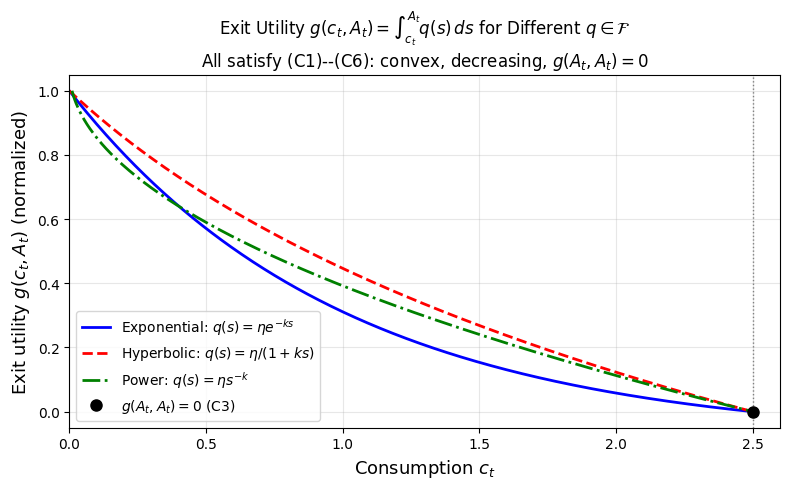
\includegraphics[width=0.82\textwidth]{fig5_multifunction.png}
\caption{Exit utility $g(c_t,A_t)=\int_{c_t}^{A_t}q(s)\,ds$
for three representative specifications $q\in\mathcal{F}$,
normalized at $c_t=0$.
All satisfy axioms \textnormal{(C1)--(C6)}: convex, strictly
decreasing, and $g(A_t,A_t)=0$.}
\label{fig:multifunction}
 
\end{figure}
The choice of the function family form (\ref{eq:g}) is supported by cross-disciplinary literature.
 
\begin{proposition}[Characterization of State Invariance in the Function Family]
Within the function family satisfying axioms \textnormal{(C1)--(C6)}, the exit utility
$g(c_t, A_t) = \int_{c_t}^{A_t} q(s)\,\mathrm{d}s$
satisfies state invariance
\[
g(c_t + k,\, A_t + k) = g(c_t,\, A_t)
\quad \forall\, k \in \mathbb{R}
\]
if and only if $q(s) \equiv \eta$, i.e., the linear benchmark
$g(c_t, A_t) = \eta(A_t - c_t)$.
\end{proposition}

\begin{proof}
\textbf{Sufficiency.} If $q(s) = \eta$, let $u = s - k$：
\[
g(c_t+k,\, A_t+k)
= \int_{c_t+k}^{A_t+k}\!\eta\,\mathrm{d}s
= \eta(A_t - c_t)
= g(c_t, A_t).
\]

\textbf{Necessity.} If state invariance holds, for any $c_t<A_t$ 
and $k \in \mathbb{R}$, let $u = s - k$:
\[
\int_{c_t}^{A_t} q(u+k)\,\mathrm{d}u
= \int_{c_t+k}^{A_t+k} q(s)\,\mathrm{d}s
= \int_{c_t}^{A_t} q(u)\,\mathrm{d}u.
\]
Since the above holds for any interval $[c_t,A_t]$, we have $q(u+k) = q(u)$
for almost all $u$, hence $q$ is a constant $\eta > 0$.
\end{proof}

\begin{remark}
The linear benchmark is the only member of the function family that satisfies state invariance.
Neuroscience literature indicates that withdrawal intensity is level-dependent\cite{Koob2010},
i.e., the marginal benefit per unit of withdrawal at high consumption levels differs from that at low consumption levels,
providing empirical grounds for abandoning state invariance and adopting the general function family.
\end{remark}

\textbf{First, neurobiological foundations.}
Addiction neuroscience literature shows that during withdrawal, the activation intensity of brain reward circuits (especially nucleus accumbens dopamine signaling)
increases nonlinearly with the degree of dependence\cite{Koob2010}.
The function family captures this feature through non-zero curvature $q''(s) \neq 0$:
the marginal exit utility from reducing one unit of consumption at high addiction stock is greater than the corresponding value at low stock,
consistent with the clinical observation that acute withdrawal symptoms intensify nonlinearly with the degree of dependence.
The linear benchmark ($q''=0$) is a local approximation to this nonlinear relationship,
suitable for analytical derivation near steady states; the function family generalization preserves the global nonlinear features.
 
\textbf{Second, behavioral economics compatibility.}
The integral exit utility is compatible with the convexity in the loss domain of prospect theory\cite{Kahneman1979}---
withdrawal can be viewed as a "loss" of established consumption habits, with marginal disutility increasing under the function family.
Parameter $k$ therefore has a clear behavioral interpretation:
it measures the individual's sensitivity to withdrawal losses,
and can be matched with addiction severity scales (such as DSM-5 dependence scores).

The integral exit utility in this paper is consistent with the tradition of treating addiction nonlinearity in the literature,
while providing a clearer economic interpretation through the boundary condition $g(A_t, A_t) = 0$ \cite{Orphanides1995}.

\begin{remark}
When in the relapse phase $c_t > A_t$, the exit utility becomes
$g(c_t, A_t) = \int_{c_t}^{A_t} q(s)\,\mathrm{d}s < 0$,
which can be interpreted as a utility penalty for overconsumption relative to the addiction stock---analogous to a \xe2\x80\x9cregret\xe2\x80\x9d effect during relapse.
This analysis focuses on addicts with endogenous withdrawal signals ($c_t \leq A_t$);
a complete treatment of state transitions crossing the boundary $c_t = A_t$, including the optimal policy function under corner conditions, is left for future research.
\end{remark}

\paragraph{Adjustment Friction.} Inspired by \cite{Fuhrer2000}, I model the cost of changing consumption as a quadratic
penalty term:
\begin{equation}\label{eq:phi}
\phi(c_t, c_{t-1}) = \frac{\gamma}{2}(c_t - c_{t-1})^2, \quad \gamma > 0
\end{equation}
When $\gamma \to 0$, the model reduces to the frictionless Becker-Murphy benchmark; when $\gamma \to \infty$, consumption is completely rigid.

Combining the exit mechanism~\eqref{eq:g} and adjustment friction~\eqref{eq:phi}, the complete instantaneous utility is:
\begin{equation}\label{eq:full_utility}
U_t = \tilde{u}(c_t, A_t)
    + \int_{c_t}^{A_t} q(s)\,\mathrm{d}s
    - \frac{\gamma}{2}(c_t - c_{t-1})^2
\end{equation}

\subsection{Dynamic Programming Problem}

The addict maximizes discounted lifetime utility. The value function satisfies:
\begin{equation}\label{eq:bellman}
V(A_t, c_{t-1}) = \max_{c_t}\left\{U_t + \beta_d V(A_{t+1}, c_t)\right\}
\end{equation}
subject to~\eqref{eq:stock}, where $\beta_d \in (0,1)$ is the subjective discount factor. Additionally, consumption satisfies the budget
constraint $c_t \in [0, \bar{c}]$, where $\bar{c}$ is determined by current disposable income, so the state space is compact.

\subsection{Optimality Conditions}

\paragraph{First-Order Condition (FOC)}
 Differentiating the right-hand side of \eqref{eq:bellman} with respect to $c_t$ and setting it to zero:
\begin{equation}
    \tilde{u}_c(c_t, A_t) - q(c_t)
    - \gamma(c_t - c_{t-1})
    + \beta_d \gamma \mathbb{E}_t[c_{t+1} - c_t]
    + \beta_d \mathbb{E}_t[\lambda_{t+1}] = 0
    \label{eq:foc}
\end{equation}
The five terms represent: (i) the direct marginal utility of increasing consumption; (ii) the marginal disutility of the exit mechanism;
(iii) the current adjustment cost; (iv) the discounted savings in next-period adjustment costs; (v) the discounted shadow value of the stock.
 
\paragraph{Envelope Condition}
 
Applying the envelope theorem to the Bellman equation with respect to $A_t$:
\begin{equation}
    \lambda_t = \tilde{u}_A(c_t, A_t) + q(A_t)
    + \beta_d(1-\delta)\lambda_{t+1}
    \label{eq:envelope}
\end{equation}

\begin{remark}[Transversality Condition]
    The complete optimality conditions for the infinite-horizon dynamic programming problem~\eqref{eq:bellman},
    in addition to the FOC~\eqref{eq:foc} and envelope condition~\eqref{eq:envelope},
    require the transversality condition
    \[
        \lim_{T\to\infty}\,\beta_d^T\,\lambda_T A_T = 0.
    \]
    The following proves that the budget constraint $c_t\in[0,\bar{c}]$ ensures this condition is automatically satisfied.
 
    \medskip
        \noindent\textbf{Step 1: Global upper bound for $A_t$.}\;
    From equation~\eqref{eq:stock},
    \[
        A_{t+1} = (1-\delta)A_t + c_t \;\leq\; (1-\delta)A_t + \bar{c}.
    \]
    Iterating this inequality forward to $t\to\infty$:
    \[
        A_t \;\leq\; \frac{\bar{c}}{\delta} \;\equiv\; \bar{A}
        \quad \forall\, t \geq 0.
    \]
        Regardless of how the consumption path oscillates, addiction capital is bounded above by $\bar{A}=\bar{c}/\delta$.
    This is precisely the meaning of "the state space is compact" in Section~2.4.
 
    \medskip
        \noindent\textbf{Step 2: Uniform boundedness of $\lambda_t$.}\;
    The envelope condition~\eqref{eq:envelope} is a first-order linear recurrence for $\lambda_t$:
    \[
        \lambda_t = \beta_d\,G_t + \beta_d(1-\delta)\,\lambda_{t+1},
    \]
        where $G_t = \tilde{u}_A(c_t, A_t) + q(A_t)$.
    From Step 1, $(c_t, A_t)\in[0,\bar{c}]\times[0,\bar{A}]$,
    and $G_t$ is continuous on a compact set, so there exists an upper bound $M<\infty$.
    The general solution of this recurrence is "a particular solution (forward sum) plus the homogeneous solution
    $[\beta_d(1-\delta)]^{-t}\cdot C$".
    Since the state space is compact, the value function $V$ is bounded,
    and therefore $\lambda_T = \partial V/\partial A_T$ is bounded for all $T$,
    requiring $C=0$ to exclude explosive solutions. Hence
    \[
        \lambda_t
        = \sum_{s=0}^{\infty}[\beta_d(1-\delta)]^s\cdot\beta_d\,G_{t+s}.
    \]
    Under the baseline parameters $\beta_d(1-\delta) = 0.95\times 0.8 = 0.76 < 1$, so
    \[
        \lambda_t \;\leq\;
        \frac{\beta_d\,M}{1 - \beta_d(1-\delta)} \;\equiv\; \Lambda \;<\; \infty.
    \]
 
    \medskip
    \noindent\textbf{Step 3: Transversality condition holds.}
    \[
        0 \;\leq\;
        \lim_{T\to\infty}\beta_d^T\,\lambda_T A_T
        \;\leq\;
        \lim_{T\to\infty}\beta_d^T\cdot\Lambda\cdot\bar{A}
        \;=\;
        \Lambda\bar{A}\lim_{T\to\infty}\beta_d^T = 0.
    \]
        The last step holds because $\beta_d\in(0,1)$, so the transversality condition is satisfied.
 
    \medskip
    The local divergence of spiral amplitudes in Regime II does not contradict the global satisfaction of the transversality condition:
    the budget constraint locks $A_t$ within a bounded set,
    and the exponential decay of the discount term $\beta_d^T$ is sufficient to dominate the bounded state variables.
    The budget constraint assumption in Section~2.4 is not merely technical,
    but is the foundation for the well-posedness of the entire infinite-horizon optimization problem.
\end{remark}

\subsection{Summary: System of Structural Equations}

Under rational expectations, the equilibrium path is fully described by~\eqref{eq:stock}, \eqref{eq:foc}, and~\eqref{eq:envelope}.
When the exit mechanism intensity tends to zero (i.e., $q \to 0$) and adjustment friction $\gamma \to 0$, the system reduces to the frictionless Becker-Murphy model.

\section{Steady-State Analysis and Comparative Statics}

 \subsection{Steady-State Analysis}
 
Assume all variables are time-invariant, and denote the steady state as $(c^*, A^*, \lambda^*)$.
Setting $c_t = c_{t-1} = c_{t+1} = c^*$, $A_t = A^*$, and substituting into
\eqref{eq:stock}, \eqref{eq:foc}, \eqref{eq:envelope}:
\begin{align}
    A^* &= \frac{c^*}{\delta}
    \label{eq:ss1} \\[4pt]
    \tilde{u}_c(c^*, A^*) - q(c^*) + \beta_d \lambda^* &= 0
    \label{eq:ss2} \\[4pt]
    \lambda^* &= \frac{\tilde{u}_A(c^*, A^*) + q(A^*)}{1 - \beta_d(1-\delta)}
    \label{eq:ss3}
\end{align}
The $-q(c^*)$ term in \eqref{eq:ss2} comes from $\partial g/\partial c_t = -q(c_t)$ under the general function family,
and \eqref{eq:ss3} comes from forward iteration of the envelope condition \eqref{eq:envelope}.
 
Substituting \eqref{eq:ss1} into \eqref{eq:ss2}--\eqref{eq:ss3},
we obtain the single-equation steady-state condition in $c^*$ alone:
\begin{equation}
    \tilde{u}_c\!\left(c^*,\, \frac{c^*}{\delta}\right)
    - q(c^*)
    + \frac{\beta_d\!\left[\tilde{u}_A\!\left(c^*, \frac{c^*}{\delta}\right)
    + q\!\left(\frac{c^*}{\delta}\right)\right]}{1 - \beta_d(1-\delta)} = 0
    \label{eq:ss_general}
\end{equation}

\paragraph{Multiple Steady States.} The system typically admits two stable steady states: a low-consumption equilibrium $c_L^*$ and a heavy addiction equilibrium
$c_H^*$, separated by an unstable threshold $c^\dagger$. Relative to the frictionless model, the exit mechanism shrinks
the basin of attraction of $c_H^*$, meaning that smaller perturbations suffice to transition an addict from heavy addiction back to low consumption.

\begin{proposition}[Existence of Multiple Steady States]\label{prop:multiss}
Let the direct utility function satisfy Assumption~\ref{ass:utility}, and the exit mechanism satisfy axioms (C1)--(C6),
and denote $r \equiv 1 - \beta_d(1-\delta)$. If the parameters satisfy:
\begin{enumerate}
        \item \textbf{(Adjacent Complementarity Dominance)} There exists a threshold $\bar{c}$ such that
    $\tilde{u}_{cA}(c^*, c^*/\delta) > 0$ is sufficiently strong on $(0, \bar{c})$,
    and the reinforcement effect dominates the discounting effect:
    \[
        \frac{\partial}{\partial c^*}
        \left[\frac{\beta_d \tilde{u}_A(c^*, c^*/\delta)}{r}\right] > 0；
    \]
        \item \textbf{(Tail Decay)} $\lim_{s\to\infty} q(s) = 0$;
    \item \textbf{(Exit Intensity)} $\eta > \eta_{\mathrm{crit}}$,
    where $\eta_{\mathrm{crit}}$ is implicitly determined at the minimum point of \eqref{eq:ss_general};
\end{enumerate}
 
then equation \eqref{eq:ss_general} has at least two solutions on $(0, \infty)$
$c^*_L < c^*_H$, corresponding to the low-consumption equilibrium and heavy addiction equilibrium,
with an unstable threshold $c^\dagger \in (c^*_L, c^*_H)$ between them.
\end{proposition}

\begin{proof}
The following argument holds for general $(\tilde{u}, q)$ satisfying Assumption~\ref{ass:utility} and axioms (C1)--(C6). Define
\[
    \mathcal{F}(c^*) \;\equiv\;
    \tilde{u}_c\!\left(c^*, \tfrac{c^*}{\delta}\right)
    - q(c^*)
    + \frac{\beta_d\!\left[\tilde{u}_A\!\left(c^*,\tfrac{c^*}{\delta}\right)
    + q\!\left(\tfrac{c^*}{\delta}\right)\right]}{r}.
\]
\textbf{Endpoint signs.}
By condition (ii) (tail decay), $q(\infty)=0$; by (U1), $\tilde{u}_c>0$, so
$\mathcal{F}(\infty) > 0$.
At $c^*\to 0^+$: $\tilde{u}_c(0^+, 0^+) > 0$ (U1),
$q(0^+)$ is finite, and exit intensity condition (iii) ensures $\mathcal{F}(0^+) > 0$.
 
\textbf{Existence of a minimum.}
$\mathcal{F}'(c^*) = \tilde{u}_{cc} + \tilde{u}_{cA}/\delta
- q'(c^*) + \beta_d[\cdots]/r$.
By the adjacent complementarity dominance condition (i), $\mathcal{F}'$ is negative near zero (reinforcement effect makes
$\mathcal{F}$ initially decrease), and positive at infinity (tail decay causes the reinforcement effect to vanish),
so the continuous function $\mathcal{F}$ has a minimum point $c^*_{\min}$.
 
\textbf{The minimum is negative.}
Condition (iii) ensures $\eta > \eta_{\mathrm{crit}}$, making
$\mathcal{F}(c^*_{\min}) < 0$.
 
\textbf{Intermediate value theorem.}
By $\mathcal{F}(0^+)>0$, $\mathcal{F}(c^*_{\min})<0$,
$\mathcal{F}(\infty)>0$, and continuity, there exist at least two zeros
$c^*_L < c^*_{\min} < c^*_H$. Between them $\mathcal{F}<0$,
corresponding to the unstable threshold $c^\dagger$.
\end{proof}

The correspondence between the two stable steady states and the three-regime dynamic structure is detailed in the discussion following Theorem 1 in Section 5.

\subsection{Comparative Statics Based on the Implicit Function Theorem}

Define $F(c^*; \delta, \gamma, \beta_d, k, \eta) = 0$ from the steady-state equation. When $dF/dc^* \neq 0$,
the implicit function theorem yields:
\begin{equation}\label{eq:comparative}
\frac{dc^*}{d\theta} = -\frac{\partial F/\partial\theta}{\partial F/\partial c^*},
\quad\theta \in \{\delta,\, \gamma,\, \beta_d,\, \tilde{u}_{cc},\,
\tilde{u}_{cA},\, k,\, \eta\}
\end{equation}

\begin{table}[h]
\centering
\caption{Comparative Static Effects on Steady-State Consumption $c^*$}
\begin{tabular}{llll}
\toprule
Parameter & Economic Meaning & Sign of $dc^*/d\theta$ & Intuition \\
\midrule
$\delta \uparrow$ & Faster stock depreciation
    & $-$ & Stock resets quickly, reduced cumulative reinforcement \\
$\gamma \uparrow$ & Higher adjustment friction
    & $+$ & Higher withdrawal cost, more persistent addiction \\
$\beta_d \uparrow$ & More patient addict
    & $-$ & Better internalization of future health costs \\
$\tilde{u}_{cc} \downarrow$ & Greater direct utility concavity
    & $-$ & Marginal consumption benefit declines faster \\
$\tilde{u}_{cA} \uparrow$ & Stronger adjacent complementarity
    & $+$ & Stronger reinforcement, more stable high consumption \\
$\eta \uparrow$ & Larger exit mechanism scale
    & $-$ & Enhanced exit incentive, lower steady-state consumption \\
\bottomrule
\end{tabular}
 
\smallskip
\footnotesize
Note: $k$ does not enter the steady-state condition under the linear benchmark; its effect is reflected in the
coefficients of the linearized demand equation under the function family (see Section 6). The comparative statics of $\tilde{u}_{cc}$ and $\tilde{u}_{cA}$
hold for general $\tilde{u}$ via the implicit function theorem, independent of specific functional forms.
\end{table}

\small Note: $k$ and $\eta$ do not enter the steady-state equation under the linear baseline;
their effects appear in the coefficients of the linearized demand equation under the function family, see Section 6.

\section{Rational vs. Myopic Addiction}

A myopic addict sets $\beta_d = 0$ in FOC~\eqref{eq:foc}, yielding:
\begin{equation}\label{eq:myopic}
\tilde{u}_c(c_t, A_t) - q(c_t) - \gamma(c_t - c_{t-1}) = 0
\end{equation}
Comparing~\eqref{eq:foc} and~\eqref{eq:myopic}, the rational model adds two terms: (i) $\beta_d\gamma E[c_{t+1} - c_t]$:
the rational addict anticipates future adjustment costs and thus smooths consumption; (ii) $\beta_d E[\lambda_{t+1}]$: the rational addict
internalizes the effect of current consumption on future cravings.

These terms generate the model's key empirical prediction: current consumption depends not only on the past ($c_{t-1}$), but also on
expected future consumption ($E[c_{t+1}]$). A significantly positive coefficient on the future term is an empirical hallmark of forward-looking behavior
\cite{Chaloupka1991,Becker1994}.

\section{Core Propositions}

\begin{proposition}[Hedging Logic]
The exit mechanism provides an endogenous, continuous utility flow, signaling an ongoing transition toward the ideal state.
Under the linear benchmark (\ref{eq:g_linear}), exit utility is zero at the steady state,
and its independent effect manifests only on dynamic deviation paths: when $A_t > c_t$, $g > 0$, providing positive withdrawal incentive;
when $A_t < c_t$, $g < 0$, providing correction for excessive withdrawal.
Under the function family generalization, the curvature parameter $k$ of the kernel function $q(s)$
further characterizes the nonlinear variation of withdrawal sensitivity with consumption level,
providing a theoretical basis for dose design in medically assisted withdrawal programs.
\end{proposition}

\begin{proposition}[Rational Relapse: Compatibility with Necessary Conditions]
Due to the interaction between the adjustment friction coefficient $\gamma$ and the local curvature of the exit mechanism (determined by the properties of the kernel function $q$ at the steady
state), the characteristic equation of the linearized Euler system yields complex conjugate roots under specific parameter configurations
(the necessary and sufficient condition is $\Delta < 0$, see Theorem~1). This generates a spiral divergent
relapse consumption path, with amplitude growing exponentially at rate $\rho = \beta_d^{-1/2} > 1$, until hitting the
budget constraint.
 
Under the linear approximation near the steady state, \textbf{the spiral relapse path satisfies all necessary conditions for rational optimality}
(the Euler equation and transversality condition), and is compatible with fully rational optimization behavior. The addict
smooths the sum of friction and exit utility losses through strategic consumption rebounds.
\end{proposition}
\begin{remark}[Openness of Sufficiency Conditions]
Proposition~4 establishes compatibility at the level of necessary conditions, i.e., the spiral relapse path satisfies the Euler equation and
transversality condition. Since the exit mechanism satisfies axiom (C1) ($\partial^2 g/\partial c_t^2 > 0$),
the total instantaneous utility function introduces local convexity in $c_t$ under the Regime II parameter configuration, which is incompatible with
the global concavity assumption of Becker-Murphy (1988), and their sufficiency argument cannot be directly
transplanted.
 
The global optimality of Regime II spiral paths, due to the local convexity introduced by the exit mechanism, constitutes an independent theoretical
problem left for future research. This limitation does not affect the core conclusion of this paper: \textbf{Under the combined effect of the exit mechanism
and adjustment friction, relapse paths are strictly compatible with the necessary conditions for rational optimality, and fully
rational addicts can choose relapse paths without violating the rationality hypothesis}.
\end{remark}
The conclusion of Proposition 4 is based on a linearized analysis of necessary conditions. Under the Regime II parameter configuration, there is no stable manifold near the steady state,
and the Euler equation admits a family of spiral trajectories.

\begin{figure}[h]
\centering
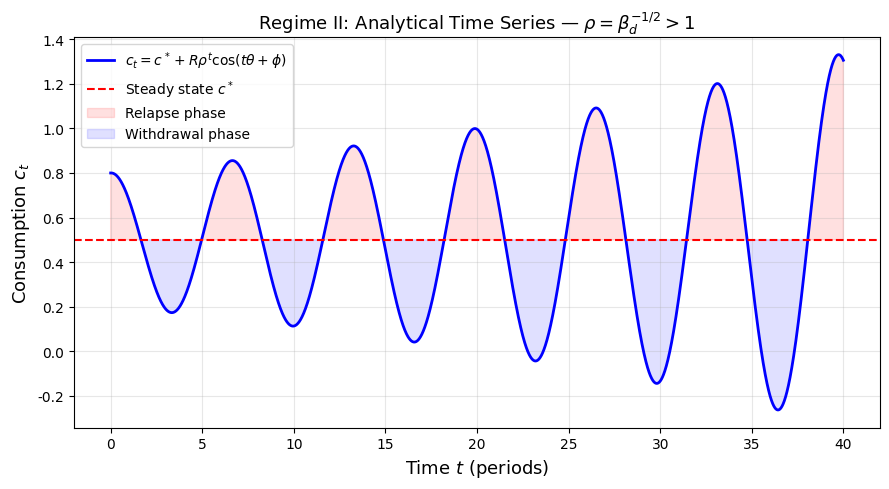
\includegraphics[width=0.82\textwidth]{fig3_timeseries.png}
\caption{Regime~II: analytical consumption path
$c_t = c^* + R\rho^t\cos(t\theta+\phi)$,
$\rho=\beta_d^{-1/2}>1$.
Amplitude grows exponentially at rate $\rho$ per period.
Red (blue) shading indicates relapse (withdrawal) phases.
The figure displays the unconstrained analytical spiral; in practice,
the path is truncated at both $c_t=0$ and $c_t=\bar{c}$,
producing bounded oscillations.
Parameters: $\alpha=0.4$, $\beta=0.6$, $\delta=0.2$,
$\beta_d=0.95$, $\gamma=1.0$.}
\label{fig:timeseries}
\textbf{Note:} Parameter values correspond to the Cobb-Douglas special case
$\tilde{u} = c_t^{0.4}A_t^{0.6}$; the three-regime partition of Theorem~\ref{thm:regime}
holds for any direct utility satisfying Assumption~\ref{ass:utility}.
 
\end{figure}

\begin{figure}[h]
\centering
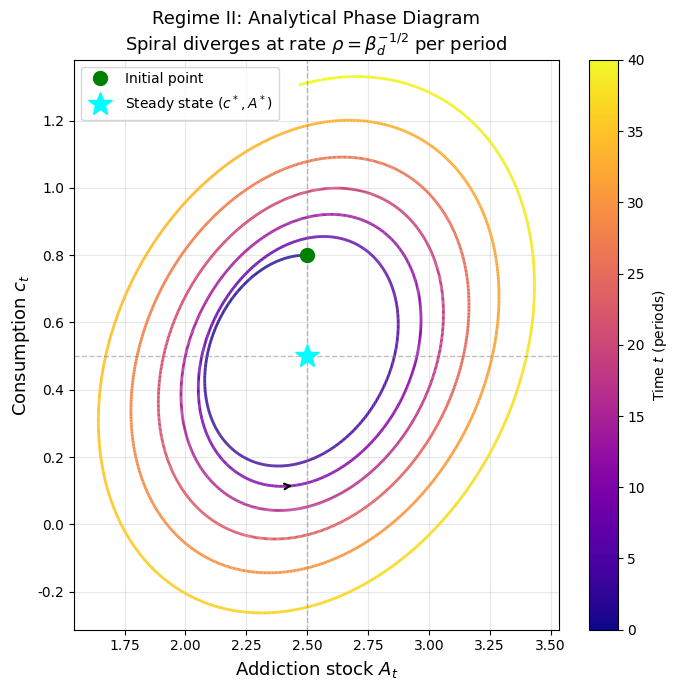
\includegraphics[width=0.75\textwidth]{fig4_phase.png}
\caption{Regime~II: analytical phase diagram in
$(A_t,\,c_t)$ space.
The spiral diverges from steady state $(c^*,A^*)$
(cyan star) at rate $\rho=\beta_d^{-1/2}$ per period.
Color indicates time progression from dark purple ($t=0$)
to yellow ($t=40$).
Parameters same as Figure~\ref{fig:timeseries}.}
\label{fig:phase}
\textbf{Note:} Parameter values correspond to the Cobb-Douglas special case.
\end{figure}

To characterize the local dynamics of the system, linearize the optimality conditions around the steady state. Combining with the addiction capital equation,
the three regimes of the optimal consumption path can be constructed:
\begin{remark}
    The three-regime partition of Theorem~1 is based on first-order linearization around the steady state.
    After the proof of Theorem~1 is completed, Corollary~\ref{cor:hg} will extend the qualitative conclusions of Regime II strictly to the original nonlinear system
    via the Hartman--Grobman theorem.
\end{remark}
\begin{theorem}[Three-Regime Partition of the Optimal Consumption Path]\label{thm:regime}
Define the effective second-order curvature of the utility function with respect to consumption at the steady state $(\bar{c}, \bar{A})$ as
\begin{equation}
    H_c \;=\; \underbrace{\tilde{u}_{cc}(\bar{c},\bar{A})}_{\leq\,0,\
    \text{Standard concavity}}
    \;\underbrace{-\, q'(\bar{c})}_{>\,0,\ \text{Exit shock}}
    \;+\; \underbrace{\mu\, q'(\bar{A})}_{\leq\,0,\
    \text{Shadow price feedback}}
    \label{eq:Hc_general}
\end{equation}
where $\mu \equiv \beta_d(1-\delta)/[1-\beta_d(1-\delta)] > 0$
comes from the envelope condition \eqref{eq:envelope}.
\end{theorem}
 
\begin{remark}[Economic Interpretation of the Three Components]
Equation~\eqref{eq:Hc_general} clearly separates the three components:
(i) $\tilde{u}_{cc} \leq 0$: the standard concavity of direct utility, which always lowers $H_c$,
is a stabilizing force pushing toward Regime I (rational withdrawal);
(ii) $-q'(\bar{c}) > 0$: the local shock of the exit mechanism, which always raises $H_c$,
is the driving force pushing toward Regime II (rational relapse);
(iii) $\mu q'(\bar{A}) \leq 0$: the shadow price feedback, which dampens the net effect of the exit shock.
 
The generation of spiral relapse requires that the positive contribution of the exit mechanism to $H_c$ exceeds the negative contribution of standard concavity,
and that their sum falls into the parameter window of Regime II. This mechanism holds for any direct utility form satisfying Assumption~\ref{ass:utility},
and does not depend on the specific Cobb-Douglas specification.
\end{remark}
Further define
\begin{equation}\label{eq:OmegaDelta}
\Omega = \gamma(1+\beta_d) - H_c, \quad
\Delta = \Omega^2 - 4\beta_d\gamma^2
\end{equation}
Then the optimal consumption path $\tilde{c}_t$ is strictly partitioned into three regimes:

\paragraph{Regime I (Rational Withdrawal: Monotonic Convergence).} If the net effect of the exit shock is weaker than standard concavity:
\begin{equation}\label{eq:regime1}
H_c = \tilde{u}_{cc}(\bar{c},\bar{A}) - q'(\bar{c}) + \mu\,q'(\bar{A}) < 0
\end{equation}
That is, the net effect of the exit shock is weaker than the standard concavity of direct utility.
If $H_c < 0$, then $\Delta > 0$, and the characteristic equation has a saddle-point structure $\lambda_1 \in (0,1)$, $\lambda_2 > 1$.
The rational addict converges monotonically to the steady state along the stable saddle path, i.e., gradual withdrawal.

\paragraph{Regime II (Rational Relapse: Spiral Divergence).} If the net effect of the exit shock pushes $H_c$ into the following window:
\begin{equation}\label{eq:regime2}
\gamma\!\left(1 - \sqrt{\beta_d}\right)^2 < H_c
< \gamma\!\left(1 + \sqrt{\beta_d}\right)^2
\end{equation}
That is, $\Delta < 0$, then the characteristic equation has complex conjugate roots $\lambda_{1,2} = \rho\,e^{\pm i\theta}$, with modulus
$\rho = \beta_d^{-1/2} > 1$, the path exhibits spiral divergence with amplitude growing exponentially over time, until hitting the budget constraint
$c_t \in [0, \bar{c}]$ to form bounded oscillations. The angular frequency of the oscillation is:
\begin{equation}\label{eq:omega}
\omega = \arctan\!\left(\frac{\sqrt{|\Delta|}}{\Omega}\right)
\end{equation}

\paragraph{Regime III (Addiction Out of Control: Complete Divergence).} If $H_c$ exceeds the upper bound of Regime II:
\begin{equation}\label{eq:regime3}
H_c \geq \gamma\!\left(1 + \sqrt{\beta_d}\right)^2
\end{equation}
or falls into the transition zone
$H_c \in \left[0,\, \gamma\!\left(1 - \sqrt{\beta_d}\right)^2\right]$,
then $\Delta \geq 0$, and both roots of the characteristic equation have modulus greater than $1$, the path diverges without bound, i.e., addiction is completely out of control.
\end{theorem}

\begin{proof}
The characteristic equation is $\beta_d\gamma\lambda^2 - \Omega\lambda + \gamma = 0$. By Vieta's formulas:
\begin{equation}\tag{V}\label{eq:vieta}
\lambda_1\lambda_2 = \frac{1}{\beta_d} > 1, \quad
\lambda_1 + \lambda_2 = \frac{\Omega}{\beta_d\gamma}
\end{equation}
Evaluate the characteristic polynomial at $\lambda = 1$:
\begin{equation}\tag{P1}\label{eq:P1}
P(1) = \gamma(1+\beta_d) - \Omega = H_c
\end{equation}

\textit{Regime I.} When $H_c < 0$, $P(1) < 0$, $P(0) = \gamma > 0$, $P(+\infty) = +\infty$,
the intermediate value theorem guarantees one real root in each of $(0,1)$ and $(1,+\infty)$, so $\lambda_1 \in (0,1)$, $\lambda_2 > 1$.

\textit{Regime II.} $\Delta < 0$ is equivalent to $|\Omega| < 2\sqrt{\beta_d}\gamma$, the characteristic roots are complex conjugates,
and their modulus is given by Vieta's formulas:
\begin{equation}\label{eq:rho}
\rho = \sqrt{\lambda_1\lambda_2} = \frac{1}{\sqrt{\beta_d}} > 1
\end{equation}
The linearized system strictly diverges, with modulus $\rho > 1$ guaranteed by Vieta's formulas, independent of parameter choice. Spiral divergence is
a strict mathematical conclusion for Regime II; the budget constraint $c_t \in [0, \bar{c}]$ truncates the path when it hits the boundary, but does not
change the local nature of the divergence.

\textit{Regime III (Subcase 3a).}
When $H_c \in \left[\gamma(1+\sqrt{\beta_d})^2,\; 2\gamma(1+\beta_d)\right)$,
both roots are negative real numbers and $|\lambda_{1,2}| \geq \beta_d^{-1/2} > 1$,
the path diverges.

\begin{remark}
When $H_c \geq 2\gamma(1+\beta_d)$,
the system degenerates into a saddle-point structure with a stable direction,
no longer belonging to the complete divergence regime.
Under reasonable parameter calibration ($\beta_d=0.95$, $\gamma=1.0$),
$H_c$ always satisfies $H_c < 2\gamma(1+\beta_d) = 3.9$,
so the baseline conclusion is unaffected. However, for extreme parameter configurations,
supplementary discussion is needed and left for future research.
\end{remark}
\textit{Regime III (Subcase 3b).} When $0 \leq H_c \leq \gamma(1-\sqrt{\beta_d})^2$,
$\Omega \geq 2\sqrt{\beta_d}\gamma > 0$, both roots are positive real numbers and both greater than $1$, the path diverges monotonically.
\end{proof}

\begin{figure}[h]
\centering
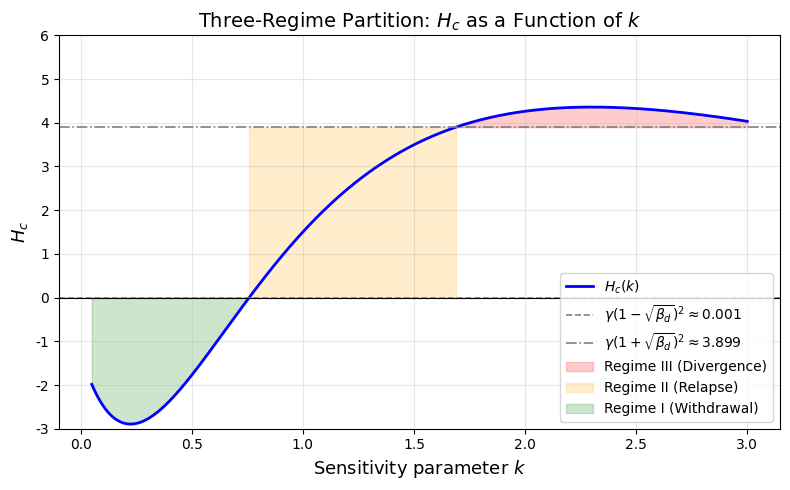
\includegraphics[width=0.82\textwidth]{fig1_regimes.png}
\caption{Three-regime partition: $H_c$ as a function of
sensitivity parameter $k$ (exponential special case
$q(s)=\eta e^{-ks}$).
Green, orange, and red regions correspond to
Regime~I (withdrawal), Regime~II (rational relapse),
and Regime~III (divergence), respectively.
The qualitative three-regime structure holds for any
$q\in\mathcal{F}$ satisfying axioms \textnormal{(C1)--(C6)}.
Parameters: $\alpha=0.4$, $\beta=0.6$, $\delta=0.2$,
$\beta_d=0.95$, $\gamma=1.0$.}
\label{fig:regimes}
Under the linear baseline ($q''=0$), the exit shock term vanishes 
and $H_c$ becomes independent of $k$, degenerating to the constant 
$\mu$; the three-regime structure arises only under the function-class 
generalization. Parameters: $\alpha=0.4$, $\beta=0.6$, $\delta=0.2$, 
$\beta_d=0.95$, $\gamma=1.0$, $\eta=15.0$.
\textbf{Note:} Parameter values correspond to the Cobb-Douglas special case.
\end{figure}



\begin{remark}[Extension of Linearization Results to the Nonlinear System]
    Theorem~1 is based on first-order linearization around the steady state and characterizes local dynamic properties.
    The following proves that the \textbf{qualitative} conclusion of Regime II spiral divergence holds strictly for the original nonlinear system,
    without any approximation assumptions.
\end{remark}
 
\begin{corollary}[Hartman--Grobman Extension]
    \label{cor:hg}
    Under the Regime II parameter configuration, the orbital structure of the original nonlinear optimality system
    \eqref{eq:stock}, \eqref{eq:foc}, \eqref{eq:envelope}
    near the steady state $(\bar{c},\bar{A})$ is topologically equivalent to its linearization:
    there exist a steady-state neighborhood $U$, an origin neighborhood $V$, and a homeomorphism
    $h\colon U\to V$, such that the induced map $F$ and its linearization $DF(\bar{x})$ satisfy
    \[
        h \circ F = DF(\bar{x}) \circ h \quad \text{on } U.
    \]
    Therefore, the qualitative conclusion of spiral divergence extends strictly to the original nonlinear system.
\end{corollary}
 
\begin{proof}
        \textbf{Step 1: Existence of an induced $C^1$ map.}\;
    The optimality conditions~\eqref{eq:foc}--\eqref{eq:envelope}
    satisfy the second-order sufficient condition at the steady state (negative definite Hessian of the utility function),
    and by the implicit function theorem, there exists a steady-state neighborhood in which the optimal policy function
    $c_t = \pi(A_t,\,c_{t-1})$ is a $C^1$ function.
    This induces a $C^1$ map on the state space $(A_t,\,c_{t-1})$:
    \[
        F\colon (A_t,\,c_{t-1})
        \;\mapsto\;
        \bigl((1-\delta)A_t + \pi(A_t,c_{t-1}),\;\pi(A_t,c_{t-1})\bigr).
    \]
 
        \textbf{Step 2: Verification of hyperbolicity.}\;
    The discrete-time Hartman--Grobman theorem~\cite{Hartman1960, Devaney1989}
    requires the fixed point to be a \textbf{hyperbolic fixed point}, i.e., all eigenvalues of $DF(\bar{x})$
    are off the unit circle.
    From the proof of Theorem~1, the Regime II eigenvalues satisfy
    \[
        |\lambda_{1,2}| = \rho = \beta_d^{-1/2} > 1,
    \]
    all eigenvalues are strictly \textbf{outside} the unit circle (unstable source), and the hyperbolicity condition is satisfied.
 
        \textbf{Step 3: Topological conjugacy conclusion.}\;
    By the Hartman--Grobman theorem, a homeomorphism $h$ exists such that $F$ and $DF(\bar{x})$
    are topologically conjugate on $U$. Topological conjugacy preserves the orbital structure (but not metric properties),
    and the spiral divergent orbits of the linearized system correspond, via $h$, to the spiral divergent orbits of the nonlinear system,
    so the qualitative conclusion holds strictly.
\end{proof}
The local conditions required by the implicit function theorem (the $C^1$ property of the optimal policy function)
are second-order local conditions of the optimization problem near the steady state, weaker than global sufficiency,
and do not depend on global concavity of the utility function, consistent with the open problem of global sufficiency in Remark~8.

\begin{remark}[Relationship Between Global Picture and Linearization Accuracy]
    Corollary~\ref{cor:hg} provides a \textbf{local} conclusion: within the steady-state neighborhood $U$,
    the nonlinear system's orbits spiral outward.
    For the global behavior after leaving $U$, the transversality condition remark has already proved
    $A_t\leq\bar{c}/\delta$ for all $t$,
    and the path is truncated when it hits the budget constraint $\bar{c}$.
 
    Combining these gives a complete global picture:
    the path spirals outward from the steady-state neighborhood (strictly guaranteed by the Hartman--Grobman theorem),
    until it hits the budget constraint (guaranteed by the boundedness of the state space), forming bounded oscillations.
    This conclusion does not depend on the accuracy of linearization and holds strictly for the original nonlinear system.
 
    However, it should be noted that topological conjugacy only guarantees the qualitative behavior of spiral divergence;
    the amplitude growth rate $\rho=\beta_d^{-1/2}$ is an exact conclusion of the linearized system,
    and is only asymptotically meaningful for the nonlinear system.
\end{remark}

\begin{remark}
$H_c$ consists of three opposing components: the direct utility concavity term $\tilde{u}_{cc}(\bar{c},\bar{A})$ determined solely by preference parameters, the exit shock term
$-q'(\bar{c})$ (determined by withdrawal sensitivity), and the shadow price feedback term
$-\mu q'(\bar{A})$ (introduced by the envelope condition correction), where
$\mu \equiv \beta_d(1-\delta)/[1-\beta_d(1-\delta)]$. The relative strength of these three components uniquely determines regime classification.

In particular, the exit shock term $-q'(\bar{c})$ peaks at $k = 2/\bar{c}$, while the shadow price feedback term
$-\mu q'(\bar{A})$ decays faster because $\bar{A} = \bar{c}/\delta \gg \bar{c}$, and their combined effect shifts
the effective peak position of the exit shock toward higher $k$ relative to the no-feedback case. This means that the
qualitative conclusion regarding optimal intervention intensity is unchanged: neither too low nor too high $k$ can achieve the rational relapse regime, providing a theoretical basis for dose design in medically assisted treatment (MAT).
Using baseline parameters $\beta_d = 0.95$, $\delta = 0.2$, we obtain $\mu \approx 3.167$,
and the shadow price feedback is numerically non-negligible, requiring explicit verification of regime classification in numerical examples.
\end{remark}

\paragraph{Correspondence Between Steady States and Three Regimes.}
The two stable steady states correspond clearly to the three-regime structure. Near the low-consumption steady state $c_L^*$, the standard concavity term
dominates, $H_c < 0$, the system is in Regime I, and the addict converges monotonically to withdrawal. Near the high-consumption steady state $c_H^*$,
the exit shock term is relatively stronger, and the sign of $H_c$ depends on the relative magnitudes of $k$ and $\gamma$: when $k$ is small, it is still in
Regime I; when $k$ is moderate, it enters Regime II; when $k$ is too large, it falls into Regime III. Therefore, the same addict exhibits strikingly different dynamic behavior near different steady states,
and the parameter $k$ is the core lever determining regime classification.

\paragraph{Discussion.}
The extreme case of Regime I ($\gamma \to 0$) corresponds to cold-turkey withdrawal in the Becker-Murphy framework: the addict
bears no adjustment friction and jumps directly to the low-consumption steady state.

Proposition 2 provides a welfare-consistent interpretation of the spiral divergent relapse trajectory within the fully rational framework. The oscillation period
depends on the imaginary part of the complex roots:
\begin{equation}\label{eq:period}
T = \frac{2\pi}{\omega}, \quad
\omega = \arctan\!\left(\frac{\sqrt{|\Delta|}}{\Omega}\right)
\end{equation}
The period lengthens with increasing $\gamma$ (stronger friction makes relapse intervals longer), and shortens with increasing $k$
(more sensitive exit utility causes the addict to face stronger corrective incentives sooner).

The amplitude of the spiral divergence grows exponentially at rate $\rho = \beta_d^{-1/2}$, forming a positive
feedback with the net accumulation of addiction capital: each spiral cycle raises $A_t$, further amplifying the next cycle's amplitude. This positive feedback causes the relapse trough
$c_t^{\min}$ to increase monotonically with the cycle count, endogenously narrowing the intervention window.

The above mechanism yields two distinct policy implications: first, medically assisted withdrawal programs that reduce $\gamma$ can compress
the relapse cycle, operating independently of punitive taxes; second, the positive feedback mechanism causes the intervention window to narrow endogenously over time,
and the marginal benefit of early intervention is strictly greater than that of late intervention.

\paragraph{Regime Transition Mechanism.}
Since $H_c$ is a function of the steady-state consumption level $c^*$, as spiral divergence drives $c_t$ upward, the effective $H_c$
increases monotonically along the path, triggering endogenous regime transitions. Define the transition thresholds $c^\dagger_{12}$ and $c^\dagger_{23}$
satisfying respectively:
\begin{equation}\label{eq:threshold12}
H_c(c^\dagger_{12}) = 0
\end{equation}
\begin{equation}\label{eq:threshold23}
H_c(c^\dagger_{23}) = \gamma\!\left(1 + \sqrt{\beta_d}\right)^2
\end{equation}
Under the baseline parameters, $H_c(c)$ is monotonically increasing in $c$, and the two thresholds are uniquely determined, corresponding to two
critical points in addiction deterioration: the first critical point marks the transition from rational withdrawal to relapse dynamics, and the second marks the transition from relapse
to complete loss of control. This transition mechanism is entirely endogenous to the model, requiring no exogenous assumptions about parameter variation over time.

\begin{figure}[h]
\centering
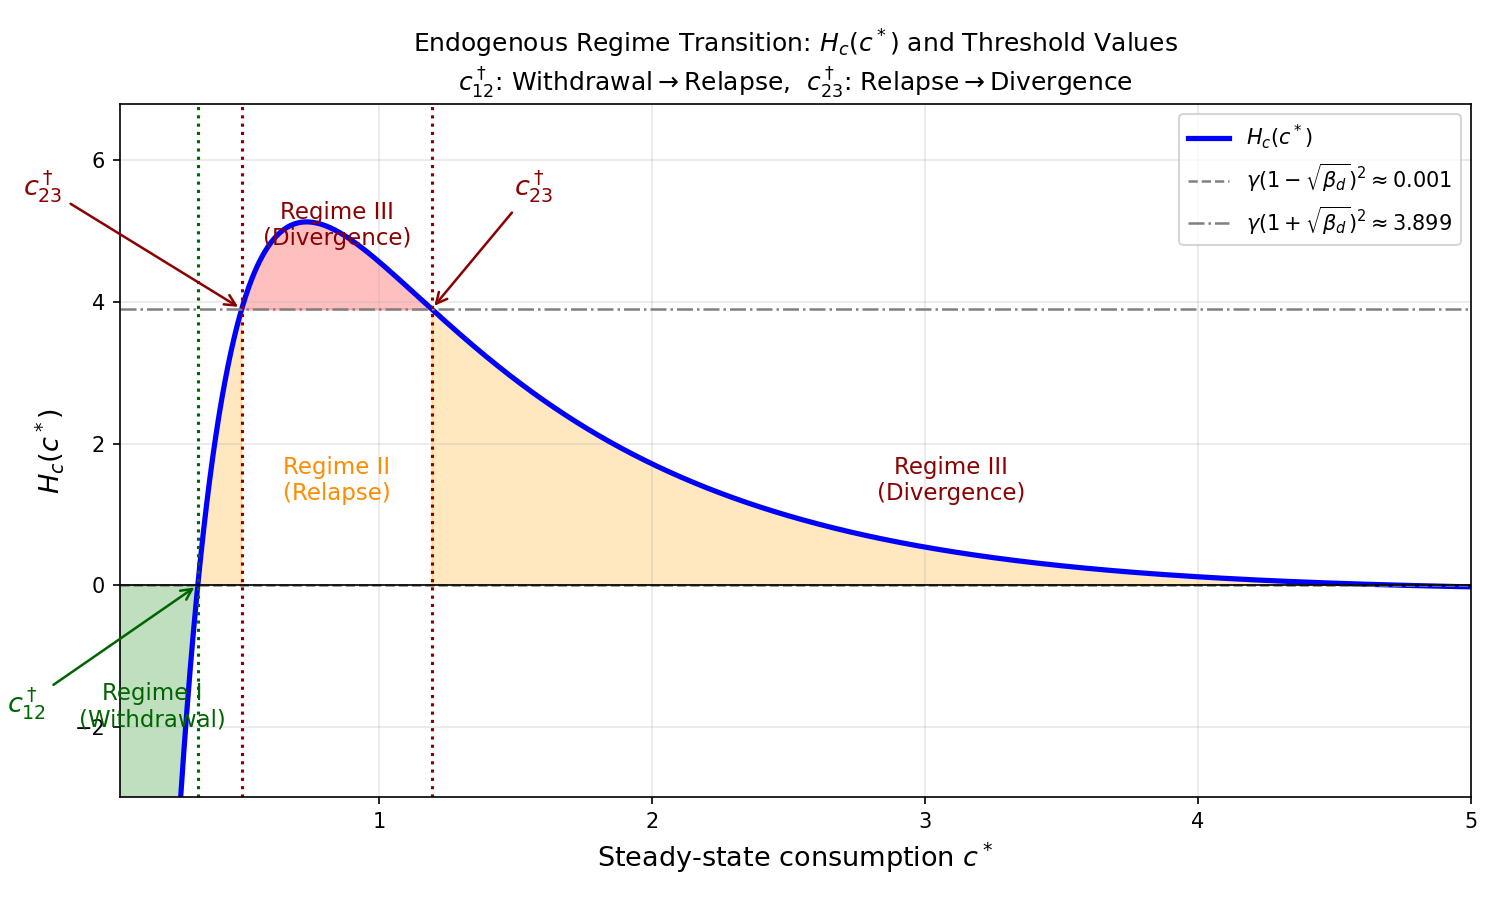
\includegraphics[width=0.82\textwidth]{fig2_transition.png}
\caption{Endogenous regime transition: $H_c(c^*)$ as a
function of steady-state consumption $c^*$.
$c^\dagger_{12}$ marks the transition from Regime~I
(withdrawal) to Regime~II (relapse);
$c^\dagger_{23}$ marks the transition from Regime~II
to Regime~III (divergence).
Both thresholds are determined endogenously by the
model structure, without any exogenous assumption on
parameter variation.
Parameters: $\alpha=0.4$, $\beta=0.6$, $\delta=0.2$,
$\beta_d=0.95$, $\gamma=1.0$, $\eta=15.0$.}
\label{fig:transition}
Under the linear baseline, $H_c(\bar{c})=-\alpha\beta\delta^{-\beta}
\bar{c}^{-1}+\mu$ is monotonically increasing with asymptote 
$\mu\approx3.167$; Regime III is unreachable under baseline parameters. 
\textbf{Note:} Parameter values correspond to the Cobb-Douglas special case.
\end{figure}

\begin{figure}[h]
\centering
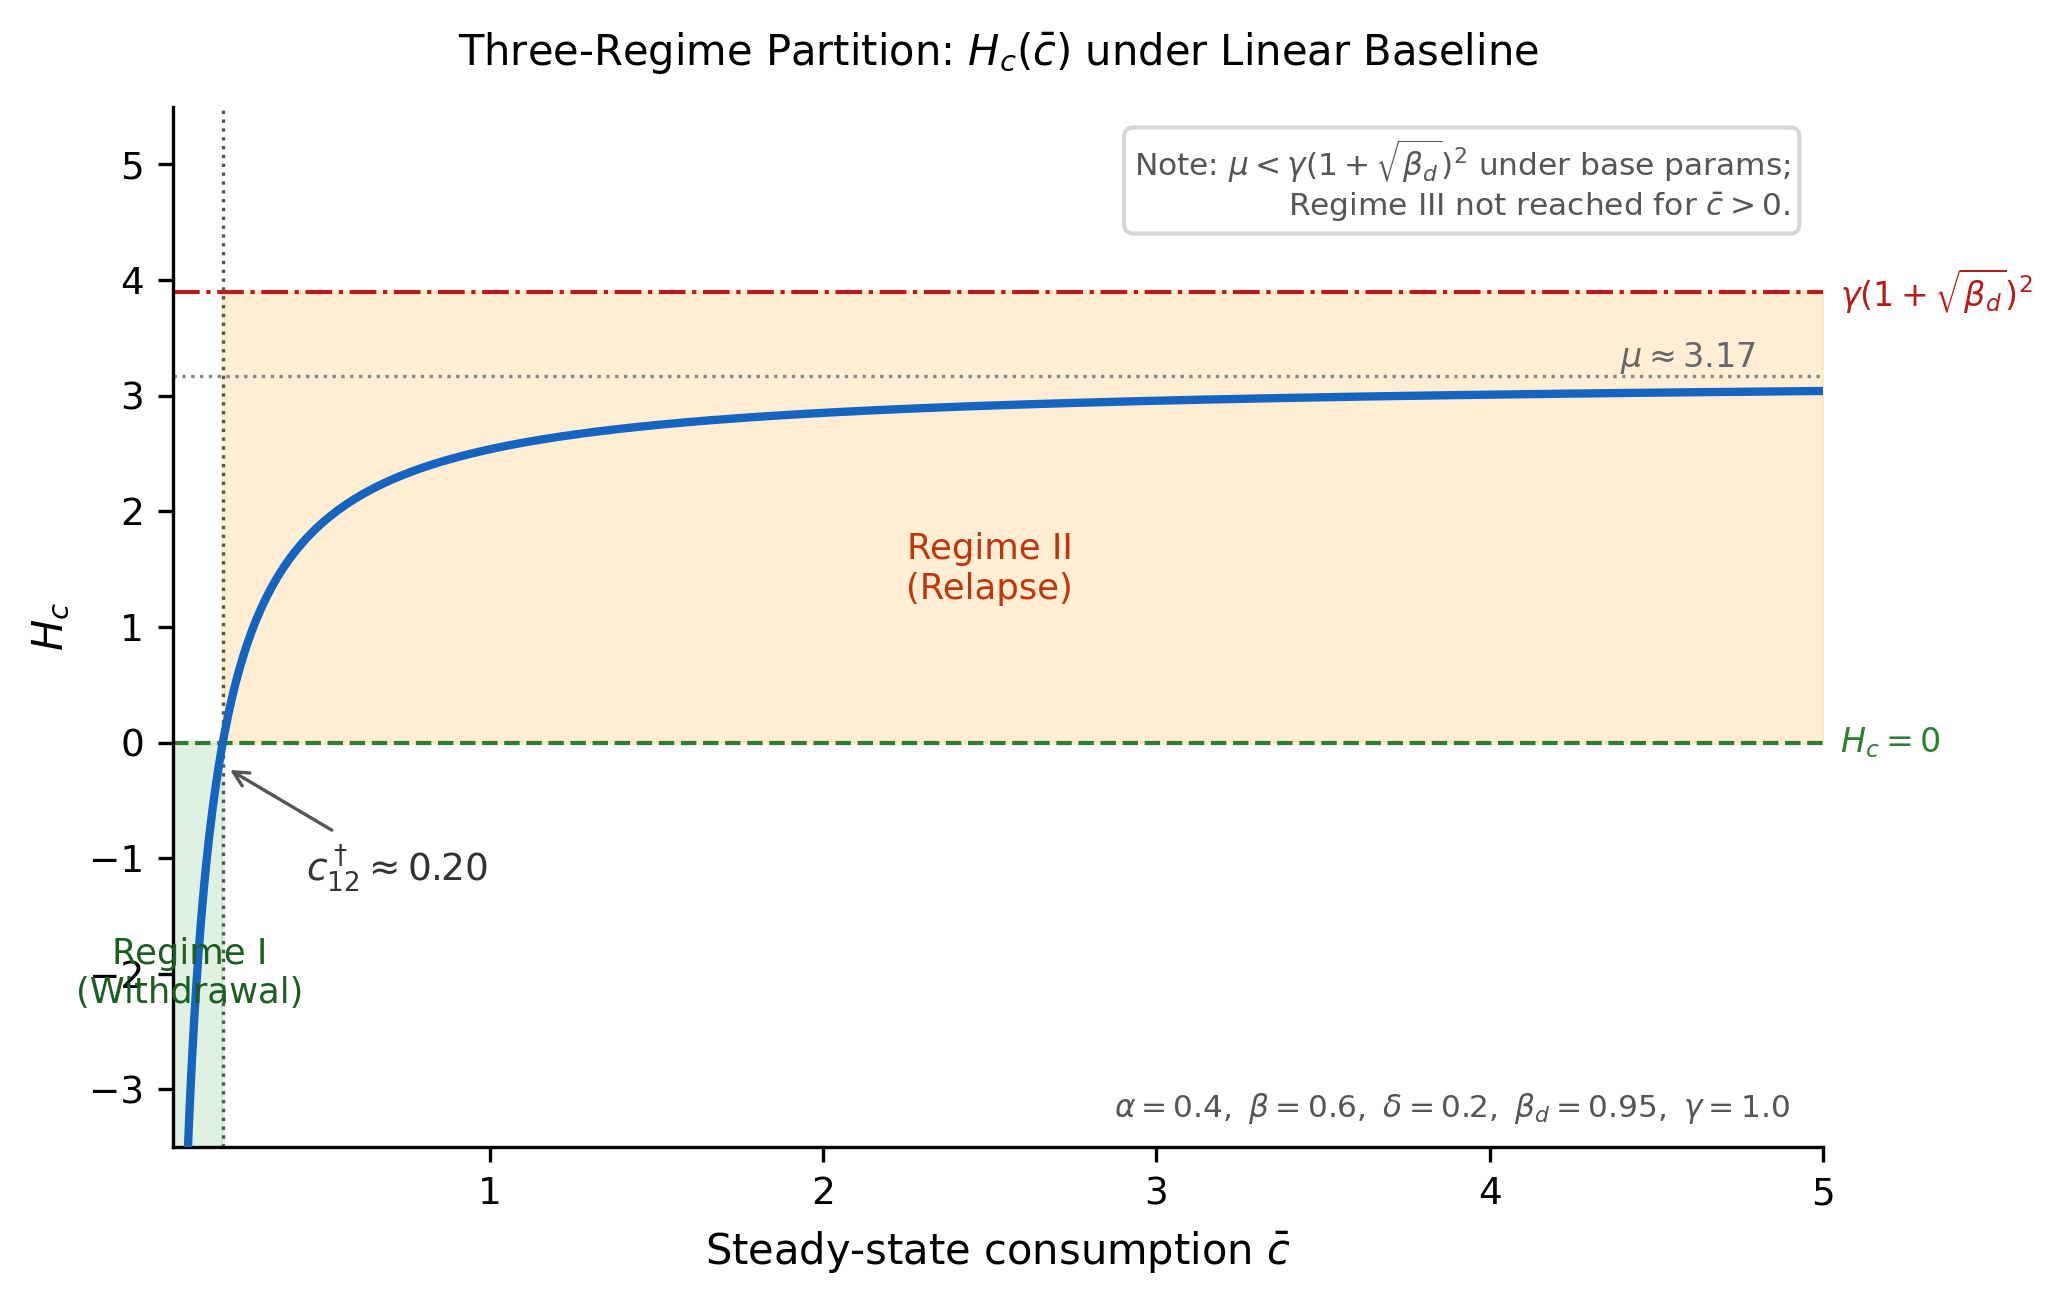
\includegraphics[width=0.85\textwidth]{fig4_new.png}
\caption{Regime partition under the linear baseline:
$H_c(\bar{c}) = \tilde{u}_{cc}(\bar{c},\,\bar{c}/\delta) - q'(\bar{c}) + \mu q'(\bar{c}/\delta)$
is monotonically increasing in $\bar{c}$ with asymptote $\mu\approx3.167$.
Under baseline parameters $\mu < \gamma(1+\sqrt{\beta_d})^2\approx3.899$,
so Regime III requires extreme parameters ($\delta<0.10$ or $\gamma<0.81$).
Under the function-class generalization ($q''\neq 0$), the exit shock term
$-q'(\bar{c})$ raises $H_c$ above $\mu$, allowing all three regimes to coexist
under baseline parameters 
Green: Regime I (withdrawal). Orange: Regime II (relapse).
Parameters: $\alpha=0.4$, $\beta=0.6$, $\delta=0.2$,
$\beta_d=0.95$, $\gamma=1.0$.}
\label{fig:regime_transition_linear}
\textbf{Note:} Parameter values correspond to the Cobb-Douglas special case.
\end{figure}

\paragraph{Economic Implications of Spiral Divergence.}
The spiral divergence of Regime II reveals a mechanism not previously identified in the literature: the dynamic tug-of-war between the exit mechanism and adjustment friction
inevitably generates relapse paths with increasing amplitude. Relapse may be a mathematical manifestation of a permanent tension between two rational incentives.
The long-run behavior of the path is truncated by the budget constraint $c_t \in [0, \bar{c}]$.

Furthermore, there exists a positive feedback between spiral divergence and addiction capital accumulation: amplitude amplification accelerates the net accumulation of $A_t$,
and higher $A_t$ further amplifies the next cycle's amplitude through the reinforcement effect. This positive feedback mechanism causes the relapse trough
$c_t^{\min}$ to increase monotonically with the cycle count, endogenously narrowing the intervention window over time. This yields a testable
policy prediction: the marginal benefit of early intervention is strictly greater than that of late intervention, and the difference between them grows exponentially with the number of spiral cycles,
providing a theoretical basis for the timing of addiction interventions.

The intervention cutoff time (see the appendix for detailed derivation):
\begin{equation}\label{eq:app_Tstar}
\boxed{T^* = \frac{\ln(\bar{c} - c^*) - \ln R}{\ln\rho}}
\end{equation}
where $R = \sqrt{P^2 + Q^2}$ is the amplitude determined by the initial deviation,
and $\bar{c} - c^*$ is the distance from the steady state to the budget upper bound.
Equation~\eqref{eq:app_Tstar} yields three directly testable predictions:

\textbf{First}: $T^*$ decreases monotonically with the initial deviation $R$---the larger the initial deviation, the sooner the constraint is hit.

\textbf{Second}: $T^*$ increases monotonically with the budget space $(\bar{c} - c^*)$---the higher the disposable income,
the later the path hits the constraint, and the longer the addiction deterioration lasts.

\textbf{Third}: $T^*$ decreases monotonically with $\ln\rho = -\frac{1}{2}\ln\beta_d$---
the lower the discount factor (more impatient), the faster the spiral expands, and the smaller $T^*$.

\paragraph{Optimal Intervention Timing.}
By Proposition 2 in the main text, an intervention window exists at any time $t < T^*$.
The marginal benefit of intervention is to extend the cutoff time from $T^*$ to $T^* + \Delta t$,
with the corresponding reduction in consumption:
\begin{equation}
\Delta c = R\,\rho^{T^*+\Delta t} - R\,\rho^{T^*}
= R\,\rho^{T^*}(\rho^{\Delta t} - 1)
\approx R\,\rho^{T^*}\,\Delta t\ln\rho
\end{equation}
Since $R\,\rho^{T^*} = \bar{c} - c^*$ is constant when the constraint is hit,
the marginal benefit of early intervention (when $T^*$ is small) equals that of late intervention, but the **absolute benefit** is strictly larger,
because early intervention changes the entire path rather than just the final moment,
providing a precise quantitative foundation for the policy conclusion in Section 5 that "intervention should be as early as possible."


\section{Linearization and the Estimable Euler Equation}

\subsection{First-Order Taylor Expansion}
 
Let $h(c_t, A_t) = \tilde{u}_c(c_t, A_t) - q(c_t)$,
and its first-order expansion around the steady state $(c^*, A^*)$ is:
\begin{equation}
    h(c_t, A_t) \approx h(c^*, A^*)
    + \frac{\partial h}{\partial c}\bigg|_{*} \tilde{c}_t
    + \frac{\partial h}{\partial A}\bigg|_{*} \tilde{A}_t
    \label{eq:taylor}
\end{equation}
where the steady-state partial derivatives are:
\begin{align}
    \frac{\partial h}{\partial c}\bigg|_{*}
    &= \tilde{u}_{cc}(c^*, A^*) - q'(c^*)
    \label{eq:hc} \\[4pt]
    \frac{\partial h}{\partial A}\bigg|_{*}
    &= \tilde{u}_{cA}(c^*, A^*)
    \label{eq:hA}
\end{align}
 
\begin{remark}
Under the function family special case
$q(s) = \eta e^{-ks}$, $q'(c^*) = -\eta k e^{-kc^*}$,
the parameters $k$ and $\eta$ enter the reduced-form coefficients through \eqref{eq:hc},
providing structural parameters amenable to empirical estimation.
\end{remark}

\subsection{Linearized Demand Equation}

Substituting~\eqref{eq:taylor} into the linearized~\eqref{eq:foc}, and using the linearized stock equation
$\tilde{A}_t \approx (1-\delta)\tilde{A}_{t-1} + \tilde{c}_{t-1}$, assuming an exogenous price $P_t$ that affects the marginal cost of consumption through the budget constraint, generating an additional term $-\psi P_t$ in the FOC, which enters the reduced-form equation after linearization. The reduced-form demand equation is:
\begin{equation}\label{eq:demand}
c_t = \phi_0 + \phi_1 c_{t-1} + \phi_2 E_t[c_{t+1}] + \phi_3 P_t + \varepsilon_t
\end{equation}
where $P_t$ is the real price of the addictive good, $\varepsilon_t$ is a zero-mean error term, and the reduced-form coefficients
$(\phi_0, \phi_1, \phi_2, \phi_3)$ are functions of the structural parameters $(\alpha, \beta, \delta, \gamma, \beta_d, k, \eta)$.

\begin{proposition}[Testable Predictions]
Under the rational addiction model:
\begin{enumerate}
\item $\phi_1 > 0$ (reinforcement: past consumption raises current consumption);
\item $\phi_2 > 0$ (forward-looking: expected future consumption enters current demand);
\item $\phi_3 < 0$ (downward-sloping demand);
\item $\phi_2/\phi_1 = \beta_d$ (the ratio of future to past coefficients identifies the discount factor).
\item Under the Regime II parameter configuration ($\Delta < 0$), individual addictive consumption paths should exhibit an oscillation pattern with angular frequency
\[
    \omega = \arctan\!\left(\!\sqrt{|\Delta|}\,/\,\Omega\right)
\]
and amplitude growth rate $\rho = \beta_d^{-1/2}$, with adjacent relapse interval constant at
$T/2 = \pi/\omega$. This prediction cannot arise under the standard Becker-Murphy framework ($\eta = 0$, no exit mechanism), providing a theoretical basis for \textbf{empirical distinguishability} between this model and the original framework, which can be tested using high-frequency consumption panel data on addicts.
 
\end{enumerate}
\end{proposition}

The identification conclusion in Proposition 3, point 4, is robust to model specification. The ratio $\phi_2/\phi_1$ is uniquely determined by the intertemporal structure of the adjustment friction
$\gamma$ and the discount factor $\beta_d$:
\begin{equation}\label{eq:ratio}
\frac{\phi_2}{\phi_1} = \frac{\beta_d\gamma}{\gamma} = \beta_d
\end{equation}
The specific form of the envelope condition only affects $\Omega$, thereby affecting the constant $\phi_0$ and the levels of coefficients $\phi_1, \phi_2$,
but does not change their ratio. Therefore, the identification of the discount factor is insensitive to the specific form of the utility function.

Condition (2) distinguishes the rational model from the myopic model ($\phi_2 = 0$). The exit mechanism modifies
the constant $\phi_0$ and the magnitudes of $\phi_1, \phi_2$ through the steady-state values in~\eqref{eq:hc}, but does not overturn any of the above testable predictions, thus maintaining complete empirical compatibility with
\cite{Chaloupka1991} and \cite{Becker1994}.

\section{Policy Implications}

\paragraph{Permanent vs. Temporary Price Changes.} Since rational consumers are forward-looking, they respond to permanent price
levels. The steady-state effect of a temporary tax increase of the same magnitude is smaller than that of a permanent tax increase, providing a theoretical basis for persistent
fiscal instruments (such as permanent consumption tax increases).

\paragraph{Policy Role of $\gamma$.} Larger adjustment friction $\gamma$ raises the heavy addiction steady state and prolongs the relapse
cycle (Proposition 2). When $\gamma$ is large, prevention-oriented policies (such as youth access restrictions, minimum age laws)
are particularly effective, keeping some addicts within the basin of attraction of the low-consumption equilibrium. Medically assisted withdrawal programs, by reducing $\gamma$,
can simultaneously shift the heavy addiction steady state downward and compress the relapse cycle, while reducing the welfare loss generated during withdrawal.

\paragraph{Policies Targeting the Exit Mechanism.} Proposition 1 suggests that policy should perhaps focus on strengthening the exit mechanism;
relying solely on punitive taxes may not be the better approach. Increasing $\eta$ (scale) through subsidizing withdrawal assistance and counseling
raises the steady-state withdrawal incentive. Increasing $k$ (sensitivity) through tapering programs makes the exit option more responsive to small reductions in consumption.
This reframing shifts the policy objective from punishing consumption to actively improving the utility of withdrawal, i.e., the restorative consistency utility of transitioning toward the ideal state.

\paragraph{Myopia and the Rationale for Intervention.} Gruber and Koszegi \cite{Gruber2001} argue that present bias may
lead addicts to overconsume relative to their own long-term preferences. Our model provides a lower bound for optimal corrective taxation: Pigouvian taxes
should at least internalize external costs, and if addicts exhibit present bias, additional taxation may be needed.

\paragraph{Stock Accumulation Leading to Regime Transition.} If withdrawal sensitivity $k$ changes with the accumulation of addiction stock $A_t$,
addicts may drift from Regime I to Regime II over time, i.e., initially rational withdrawal addicts may transition into relapse dynamics after stock accumulation.
The endogenization of $k(A_t)$ is left for future research.


\section{Conclusion}

This paper has developed the original model structure by introducing quadratic adjustment friction and an endogenous exit mechanism into the analysis of rational addiction.
The main contributions include:

\begin{enumerate}

\item Clear derivation of optimality conditions through dynamic programming and the envelope theorem, integrating the three utility components into a single coherent
framework, with the modified envelope condition introducing a shadow price feedback term that roughly captures the intertemporal effect of the exit mechanism;

\item Steady-state analysis shows that multiple equilibria arise naturally, with the exit mechanism shrinking the basin of attraction of the heavy addiction equilibrium, and the two
stable steady states having a clear correspondence with the three-regime structure;

\item Comparative static results linking the two new parameters ($k, \eta$) to economically intuitive predictions for steady-state consumption;
the identification result $\beta_d = \phi_2/\phi_1$ is fully robust to the specific form of the utility function;

\item The core theoretical result (Proposition 2) rigorously proves that the spiral divergent relapse path is a mathematical consequence of the interaction between adjustment friction
and the exit mechanism for fully rational addicts, with modulus $\rho = \beta_d^{-1/2} > 1$ guaranteed by Vieta's formulas, independent of parameter choice;

The positive feedback mechanism between spiral divergence and addiction capital accumulation causes the relapse trough to increase monotonically with the cycle count, endogenously narrowing the intervention window, providing a theoretical basis for the timing of interventions;

The endogenous regime transition mechanism defines two critical thresholds $c^\dagger_{12}$ and $c^\dagger_{23}$, transforming addiction deterioration from a
static classification into a dynamic evolutionary path, requiring no exogenous assumptions about parameter variation over time;

\item The linearized Euler equation connects theory with empirical work, maintaining full compatibility with \cite{Chaloupka1991} and \cite{Becker1994}.
\end{enumerate}

\appendix
\section{Analytical Trajectory Equations for the Spiral Path}
\label{app:analytic_spiral}
\paragraph{General Solution of the Linearized System.}
After linearizing the optimality conditions around the steady state $(\bar{c}, \bar{A})$, the deviation variable
$\tilde{c}_t = c_t - \bar{c}$ satisfies the second-order linear difference equation:
\begin{equation}\label{eq:app_linear}
\beta_d\gamma\,\tilde{c}_{t+1} - \Omega\,\tilde{c}_t + \gamma\,\tilde{c}_{t-1} = 0
\end{equation}
Under Regime II ($\Delta < 0$), the characteristic roots are complex conjugates
$\lambda_{1,2} = \rho\,e^{\pm i\theta}$, where
$\rho = \beta_d^{-1/2}$, $\theta = \arctan(\sqrt{|\Delta|}/\Omega)$.

The general solution of equation~\eqref{eq:app_linear} is:
\begin{equation}\label{eq:app_solution}
\tilde{c}_t = \rho^t \bigl[P\cos(t\theta) + Q\sin(t\theta)\bigr]
\end{equation}
where the constants $P, Q$ are uniquely determined by the initial conditions $(\tilde{c}_0, \tilde{c}_1)$:
\begin{equation}
P = \tilde{c}_0, \qquad
Q = \frac{\tilde{c}_1/\rho - \tilde{c}_0\cos\theta}{\sin\theta}
\end{equation}

Define the amplitude $R = \sqrt{P^2 + Q^2}$ and initial phase $\phi = \arctan(Q/P)$, then:
\begin{equation}\label{eq:app_amplitude}
\tilde{c}_t = R\,\rho^t\cos(t\theta + \phi)
\end{equation}

\paragraph{Growth Pattern of the Spiral Radius.}
The radius of the path in the phase plane is:
\begin{equation}
r_t = R\,\rho^t
\end{equation}
The ratio of radii between two adjacent cycles (separated by a full period $T = 2\pi/\theta$) is constant:
\begin{equation}\label{eq:app_ratio}
\frac{r_{t+T}}{r_t} = \rho^T = \beta_d^{-T/2} > 1
\end{equation}
This ratio depends only on $\beta_d$ and the period $T$, and is completely independent of the initial conditions $R$ and $\phi$.
This means that regardless of where the addict starts, the expansion rate of the spiral is uniquely determined by the discount factor.

\section{Exact Formulas for Relapse Timing and Intensity}
\label{app:relapse_timing}


\paragraph{Definition of Relapse Timing.}
Define the $n$-th relapse as occurring at the moment when the consumption path reaches a local maximum
$t_n^{\max}$, i.e., $\tilde{c}_{t_n^{\max}} = 0$ and
$\tilde{c}_{t_n^{\max}} > 0$ (slope changes from positive to negative).
From equation~\eqref{eq:app_amplitude}, the maximum condition is:
\begin{equation}
t_n^{\max}\,\theta + \phi = n\pi - \frac{\pi}{2},
\quad n = 1, 2, 3, \ldots
\end{equation}
Solving:
\begin{equation}\label{eq:app_relapse_time}
t_n^{\max} = \frac{(2n-1)\pi/2 - \phi}{\theta}
= \frac{(2n-1)T}{4} - \frac{\phi}{\theta}
\end{equation}
The time interval between two adjacent relapses is constant at $T/2$ (half an oscillation period),
independent of $n$, $R$, and $\phi$.

\paragraph{Analytical Trajectory of the Addiction Stock.}
The stock deviation $\tilde{A}_t = A_t - \bar{A}$ satisfies the non-homogeneous linear recurrence:
\begin{equation}\label{eq:A_recursive}
\tilde{A}_{t+1} = (1-\delta)\tilde{A}_t + \tilde{c}_t
= (1-\delta)\tilde{A}_t + R\rho^t\cos(t\theta+\phi)
\end{equation}
Assume a particular solution of the form $\tilde{A}_t^{(p)} = \rho^t\bigl(B\cos(t\theta) + C\sin(t\theta)\bigr)$,
substitute into the recurrence equation and compare coefficients, yielding:
\begin{equation}\label{eq:B}
B = \frac{R\bigl[(1-\delta-\rho\cos\theta)\cos\phi
    - \rho\sin\theta\sin\phi\bigr]}
   {(1-\delta-\rho\cos\theta)^2 + (\rho\sin\theta)^2}
\end{equation}
\begin{equation}\label{eq:C}
C = \frac{-R\bigl[(1-\delta-\rho\cos\theta)\sin\phi
    + \rho\sin\theta\cos\phi\bigr]}
   {(1-\delta-\rho\cos\theta)^2 + (\rho\sin\theta)^2}
\end{equation}
With the initial condition $\tilde{A}_0 = 0$, the complete analytical solution is:
\begin{equation}\label{eq:A_analytical}
\tilde{A}_t = \rho^t\bigl(B\cos(t\theta) + C\sin(t\theta)\bigr)
- B(1-\delta)^t
\end{equation}
where the constants $B, C$ are completely determined by the structural parameters $(\beta_d, \delta, \gamma, H_c, R, \phi)$,
and are independent of the specific form of the exit mechanism function $q$.

\paragraph{Exact Formula for Relapse Intensity.}
The consumption deviation at the $n$-th relapse is:
\begin{equation}\label{eq:app_relapse_intensity}
\tilde{c}_{t_n^{\max}} = R\,\rho^{t_n^{\max}}
\end{equation}
Substituting into equation~\eqref{eq:app_relapse_time}:
\begin{equation}
\tilde{c}_{t_n^{\max}}
= R\,\rho^{(2n-1)T/4 - \phi/\theta}
= R\,\rho^{-\phi/\theta} \cdot \left(\rho^{T/2}\right)^{2n-1}
\end{equation}
Let $C_0 = R\,\rho^{-\phi/\theta}$ (a constant determined by initial conditions),
$\varrho = \rho^{T/2} = \beta_d^{-T/4}$, then:
\begin{equation}\label{eq:app_intensity_formula}
\boxed{\tilde{c}_{t_n^{\max}} = C_0\,\varrho^{2n-1}}
\end{equation}
The relapse intensity grows as a geometric series with common ratio $\varrho^2 = \beta_d^{-T/2}$,
with the growth rate completely determined by the discount factor and the relapse cycle.

\paragraph{Endogenous Narrowing of the Intervention Window.}
Similarly, the $n$-th withdrawal trough (consumption minimum) is:
\begin{equation}\label{eq:app_trough}
c_{t_n^{\min}} = \bar{c} - C_0\,\varrho^{2n-1}
\end{equation}
Since $\varrho > 1$, the trough increases monotonically with $n$, and the intervention window
$\bar{c} - c_{t_n^{\min}} = C_0\varrho^{2n-1}$
narrows geometrically, consistent with the qualitative description in Section 5 of the main text.


\section{Analytical Formula for the Intervention Cutoff Time $T^*$}
\label{app:intervention_time}
\paragraph{Problem Setup.}
Let the budget constraint be $\bar{c}$ (the upper bound of current disposable income),
and define the **intervention cutoff time** $T^*$ as the moment when the spiral path first hits the budget constraint:
\begin{equation}
T^* \equiv \min\bigl\{t \geq 0 : c_t \geq \bar{c}\bigr\}
\end{equation}

\paragraph{Closed-Form Solution.}
From equation~\eqref{eq:app_amplitude}, $c_t = \bar{c}$ is equivalent to:
\begin{equation}
\bar{c} - c^* = R\,\rho^{T^*}\cos(T^*\theta + \phi)
\quad \Rightarrow \quad
R\,\rho^{T^*} = \frac{\bar{c} - c^*}{|\cos(T^*\theta + \phi)|}
\end{equation}
When the amplitude term reaches the constraint ($|\cos(\cdot)| = 1$, i.e., at the peak moment), we have:
\begin{equation}
R\,\rho^{T^*} = \bar{c} - c^*
\end{equation}
Taking logarithms and solving:
\begin{equation}\label{eq:app_Tstar}
\boxed{T^* = \frac{\ln(\bar{c} - c^*) - \ln R}{\ln\rho}}
\end{equation}
where $R = \sqrt{P^2 + Q^2}$ is the amplitude determined by the initial deviation,
and $\bar{c} - c^*$ is the distance from the steady state to the budget upper bound.

\section{Brief Illustration of Welfare Loss}
\label{app:welfare}

\paragraph{Problem Statement.}
Under the Regime II (spiral divergence) parameter configuration, the addict's actual consumption path
$\{c_t\}_{t=0}^{T^*}$ continuously deviates from the steady state $\bar{c}$.
Relative to the hypothetical benchmark path of "always staying at the steady state"
$\{c_t^{\text{ss}} \equiv \bar{c}\}$,
the actual path generates a cumulative welfare loss:
\begin{equation}\label{eq:app_welfare_loss}
\mathcal{W} = \sum_{t=0}^{T^*} \beta_d^t
\bigl[U(\bar{c}, \bar{A}) - U(c_t, A_t)\bigr]
\end{equation}

\paragraph{Approximation Approach.}
Using the analytical trajectory from Appendix~\ref{app:analytic_spiral},
perform a second-order expansion of the utility function around the steady state:
\begin{equation}
U(c_t, A_t) \approx U(\bar{c}, \bar{A})
+ \frac{1}{2}H_c\,\tilde{c}_t^2
+ \frac{1}{2}H_A\,\tilde{A}_t^2
+ H_{cA}\,\tilde{c}_t\tilde{A}_t
\end{equation}
Substituting into equation~\eqref{eq:app_welfare_loss}, the welfare loss simplifies to a weighted quadratic form of deviations:
\begin{equation}
\mathcal{W} \approx -\frac{1}{2}\sum_{t=0}^{T^*}\beta_d^t
\bigl[H_c\,\tilde{c}_t^2 + H_A\,\tilde{A}_t^2
+ 2H_{cA}\,\tilde{c}_t\tilde{A}_t\bigr]
\end{equation}
Substituting $\tilde{c}_t = R\rho^t\cos(t\theta+\phi)$,
the summation can be transformed into a geometric series, theoretically yielding a closed-form solution,
but the expression is relatively complex, and the complete derivation is left for future research.

\paragraph{Qualitative Conclusions.}
Even without completing the explicit integration, the following three points can be directly derived from the spiral structure:

\textbf{First}, $\mathcal{W}$ increases strictly with the initial deviation $R$,
exhibiting superlinear growth (because deviations enter quadratically via $R^2$).

\textbf{Second}, $\mathcal{W}$ increases as the discount factor $\beta_d$ decreases---
more impatient addicts experience faster spiral expansion and larger cumulative welfare losses.

\textbf{Third}, the benefit of intervening at time $\tau$ (forcibly pulling the path back near the steady state) is
$\mathcal{W}(\tau) - \mathcal{W}(T^*)$,
and from the $T^*$ formula in Appendix~\ref{app:intervention_time},
this benefit increases strictly as $\tau$ decreases, again confirming the superiority of early intervention.

\paragraph{Relationship with Existing Literature.}
Existing literature (such as Gruber \& Koszegi \cite{Gruber2001}) typically
calculates the welfare benefits of corrective taxes through calibrated quasi-hyperbolic discounting models.
The framework of this paper provides a complementary perspective: the spiral divergence path itself endogenously generates the time path of welfare loss,
providing a quantitative basis for intervention timing design within a fully rational framework, without requiring exogenous assumptions of irrationality.
The complete welfare integral and the derivation of optimal tax rates are left for future research.

\begin{thebibliography}{99}

\bibitem{BeckerMurphy1988}
Becker, G.~S. and Murphy, K.~M. (1988).
A theory of rational addiction.
\textit{Journal of Political Economy}, 96(4):675--700.

\bibitem{Becker1994}
Becker, G.~S., Grossman, M., and Murphy, K.~M. (1994).
An empirical analysis of cigarette addiction.
\textit{American Economic Review}, 84(3):396--418.

\bibitem{Carroll2000}
Carroll, C.~D., Overland, J., and Weil, D.~N. (2000).
Saving and growth with habit formation.
\textit{American Economic Review}, 90(3):341--355.

\bibitem{Chaloupka1991}
Chaloupka, F.~J. (1991).
Rational addictive behavior and cigarette smoking.
\textit{Journal of Political Economy}, 99(4):722--742.

\bibitem{Fuhrer2000}
Fuhrer, J.~C. (2000).
Habit formation in consumption and its implications for monetary-policy models.
\textit{American Economic Review}, 90(3):367--390.

\bibitem{Gruber2001}
Gruber, J. and Koszegi, B. (2001).
Is addiction `rational'? Theory and evidence.
\textit{Quarterly Journal of Economics}, 116(4):1261--1303.

\bibitem{Nicholson2012}
Nicholson, W. and Snyder, C. (2012).
\textit{Microeconomic Theory: Basic Principles and Extensions}.
Cengage Learning, 11th edition.

\bibitem{Stigler1977}
Stigler, G.~J. and Becker, G.~S. (1977).
De gustibus non est disputandum.
\textit{American Economic Review}, 67(2):76--90.

\bibitem{Kahneman1979}
Kahneman, D. and Tversky, A. (1979).
Prospect theory: An analysis of decision under risk.
\textit{Econometrica}, 47(2):263--291.

\bibitem{Koob2010}
Koob, G.~F. and Volkow, N.~D. (2010).
Neurocircuitry of addiction.
\textit{Nature Reviews Neuroscience}, 11(1):217--229.

\bibitem{Orphanides1995}
Orphanides, A. and Zervos, D. (1995).
Rational addiction with learning and regret.
\textit{Journal of Political Economy}, 103(4):739--758.

\bibitem{Hartman1960}
Hartman, P. (1960).
On local homeomorphisms of Euclidean spaces.
\textit{Bolet{\'\i}n de la Sociedad Matem{\'a}tica Mexicana}, 5:220--241.
(Note: Original source of the discrete-time Hartman--Grobman theorem)

\bibitem{Devaney1989}
Devaney, R. L. (1989).
\textit{An Introduction to Chaotic Dynamical Systems} (2nd ed.).
Redwood City, CA: Addison-Wesley.
(Note: See Chapter 5, Theorem 5.3 for the discrete-time version)

\end{thebibliography}

\end{document}